% ===== SUPPLEMENTAL MATERIALS =====
\section{Supplemental Materials}
% search strategy
% data table: literature and data characteristics and sources

<<<<<<< HEAD
% ===== TABLE OF CONTENTS =====
\subsection*{Table of Contents}
\begin{itemize}
    \item \hyperref[tab:comparable_models]{Table S1: Number of comparable models by city and pathogen} \dotfill \pageref{tab:comparable_models}
    \item \hyperref[tab:joint_outbreak_probability]{Table S2: Median probability of joint outbreaks by risk threshold} \dotfill \pageref{tab:joint_outbreak_probability}
    \item \hyperref[tab:survival_median_times]{Table S3: Median time to next joint outbreak by risk threshold} \dotfill \pageref{tab:survival_median_times}
    \item \hyperref[fig:supplemental_cycle_lengths]{Figure S1: Distribution of between-year cycle lengths} \dotfill \pageref{fig:supplemental_cycle_lengths}
\end{itemize}

\clearpage

% ===== TABLES SECTION =====
\subsection{Tables}

\subsubsection{Comparable Models by City and Pathogen}
\label{subsec:comparable_models}

\begin{table}[htbp]
\centering
\caption{Table S1: Number of comparable models ($\Delta$AIC $\leq$ 10) per city and pathogen. This table illustrates the distribution of model availability across the eight study cities, highlighting the variation in the number of comparable models per city.}
\label{tab:comparable_models}
\begin{tabular}{lcc}
\toprule
\textbf{City} & \textbf{Influenza} & \textbf{RSV} \\
\midrule
\multicolumn{3}{l}{\textit{North}} \\
Beijing & 20 & 39 \\
Lanzhou & 2 & 4 \\
Xian & 2 & 3 \\
\textit{North Total} & \textit{24} & \textit{46} \\
\midrule
\multicolumn{3}{l}{\textit{South}} \\
Wuhan & 20 & 22 \\
Suzhou & 18 & 3 \\
Guangzhou & 4 & 11 \\
Wenzhou & 2 & 2 \\
Yunfu & 2 & 2 \\
\textit{South Total} & \textit{46} & \textit{40} \\
\midrule
\textbf{Grand Total} & \textbf{70} & \textbf{86} \\
\bottomrule
\end{tabular}
\end{table}

\clearpage

\subsubsection{Median Probability of Joint Outbreaks by Risk Threshold}
\label{subsec:joint_outbreak_probability}

\begin{table}[htbp]
\centering
\caption{Table S2: Median probability of joint outbreaks by city and risk threshold. Values represent the median proportion of years with concurrent high-risk periods for both Influenza and RSV across 1000 simulation paths. Risk thresholds are defined as joint top 30\%, 20\%, and 10\% percentiles of disease burden.}
\label{tab:joint_outbreak_probability}
\begin{tabular}{lccc}
\toprule
\textbf{City} & \textbf{Top 30\%} & \textbf{Top 20\%} & \textbf{Top 10\%} \\
\midrule
\multicolumn{4}{l}{\textit{North}} \\
Beijing & 0.200 & 0.100 & 0.000 \\
Lanzhou & 0.118 & 0.059 & 0.000 \\
Xian & 0.450 & 0.350 & 0.150 \\
\midrule
\multicolumn{4}{l}{\textit{South}} \\
Wuhan & 0.400 & 0.300 & 0.150 \\
Suzhou & 0.350 & 0.200 & 0.100 \\
Guangzhou & 0.188 & 0.125 & 0.062 \\
Wenzhou & 0.812 & 0.500 & 0.250 \\
Yunfu & 0.375 & 0.188 & 0.125 \\
\bottomrule
\end{tabular}
\end{table}

\clearpage

\subsubsection{Median Time to Next Joint Outbreak by Risk Threshold}
\label{subsec:survival_median_times}

\begin{table}[htbp]
\centering
\caption{Table S3: Median time to next joint outbreak (years) by city and risk threshold, with 95\% confidence intervals. Values represent the x-intercepts of the dashed vertical lines in Figure 5, indicating the time (in years) at which 50\% of simulation paths are expected to experience their next joint outbreak. Confidence intervals (in parentheses) reflect uncertainty in the Kaplan-Meier survival estimates, which properly account for right-censoring of paths that never experience a second outbreak. The relatively narrow confidence intervals reflect high precision from aggregating across 1000 simulation paths per city. Values marked as ``---'' indicate that the 50\% threshold was not reached within the simulation window. Risk thresholds are defined as joint top 30\%, 20\%, and 10\% percentiles of disease burden.}
\label{tab:survival_median_times}
\begin{tabular}{lccc}
\toprule
\textbf{City} & \textbf{Top 30\%} & \textbf{Top 20\%} & \textbf{Top 10\%} \\
\midrule
\multicolumn{4}{l}{\textit{North}} \\
Beijing & 3.0 (2.0--3.0) & 5.0 (4.0--6.0) & --- \\
Lanzhou & 5.0 (5.0--6.0) & --- & --- \\
Xian & 1.0 (1.0--1.0) & 2.0 (2.0--2.0) & 3.0 (3.0--3.0) \\
\midrule
\multicolumn{4}{l}{\textit{South}} \\
Wuhan & 1.0 (1.0--1.0) & 2.0 (2.0--2.0) & 3.0 (3.0--3.0) \\
Suzhou & 2.0 (2.0--2.0) & 3.0 (3.0--3.0) & 6.0 (5.0--6.0) \\
Guangzhou & 3.0 (3.0--4.0) & 6.0 (6.0--7.0) & --- \\
Wenzhou & 1.0 (1.0--1.0) & 1.0 (1.0--1.0) & 2.0 (2.0--2.0) \\
Yunfu & 2.0 (2.0--2.0) & 3.0 (3.0--3.0) & 7.0 (6.0--8.0) \\
\bottomrule
\end{tabular}
\end{table}

\clearpage

% ===== FIGURES SECTION =====
\subsection{Figures}

\subsubsection{Distribution of Between-Year Cycle Lengths}
\label{subsec:cycle_lengths}

\begin{figure}[htbp]
\centering
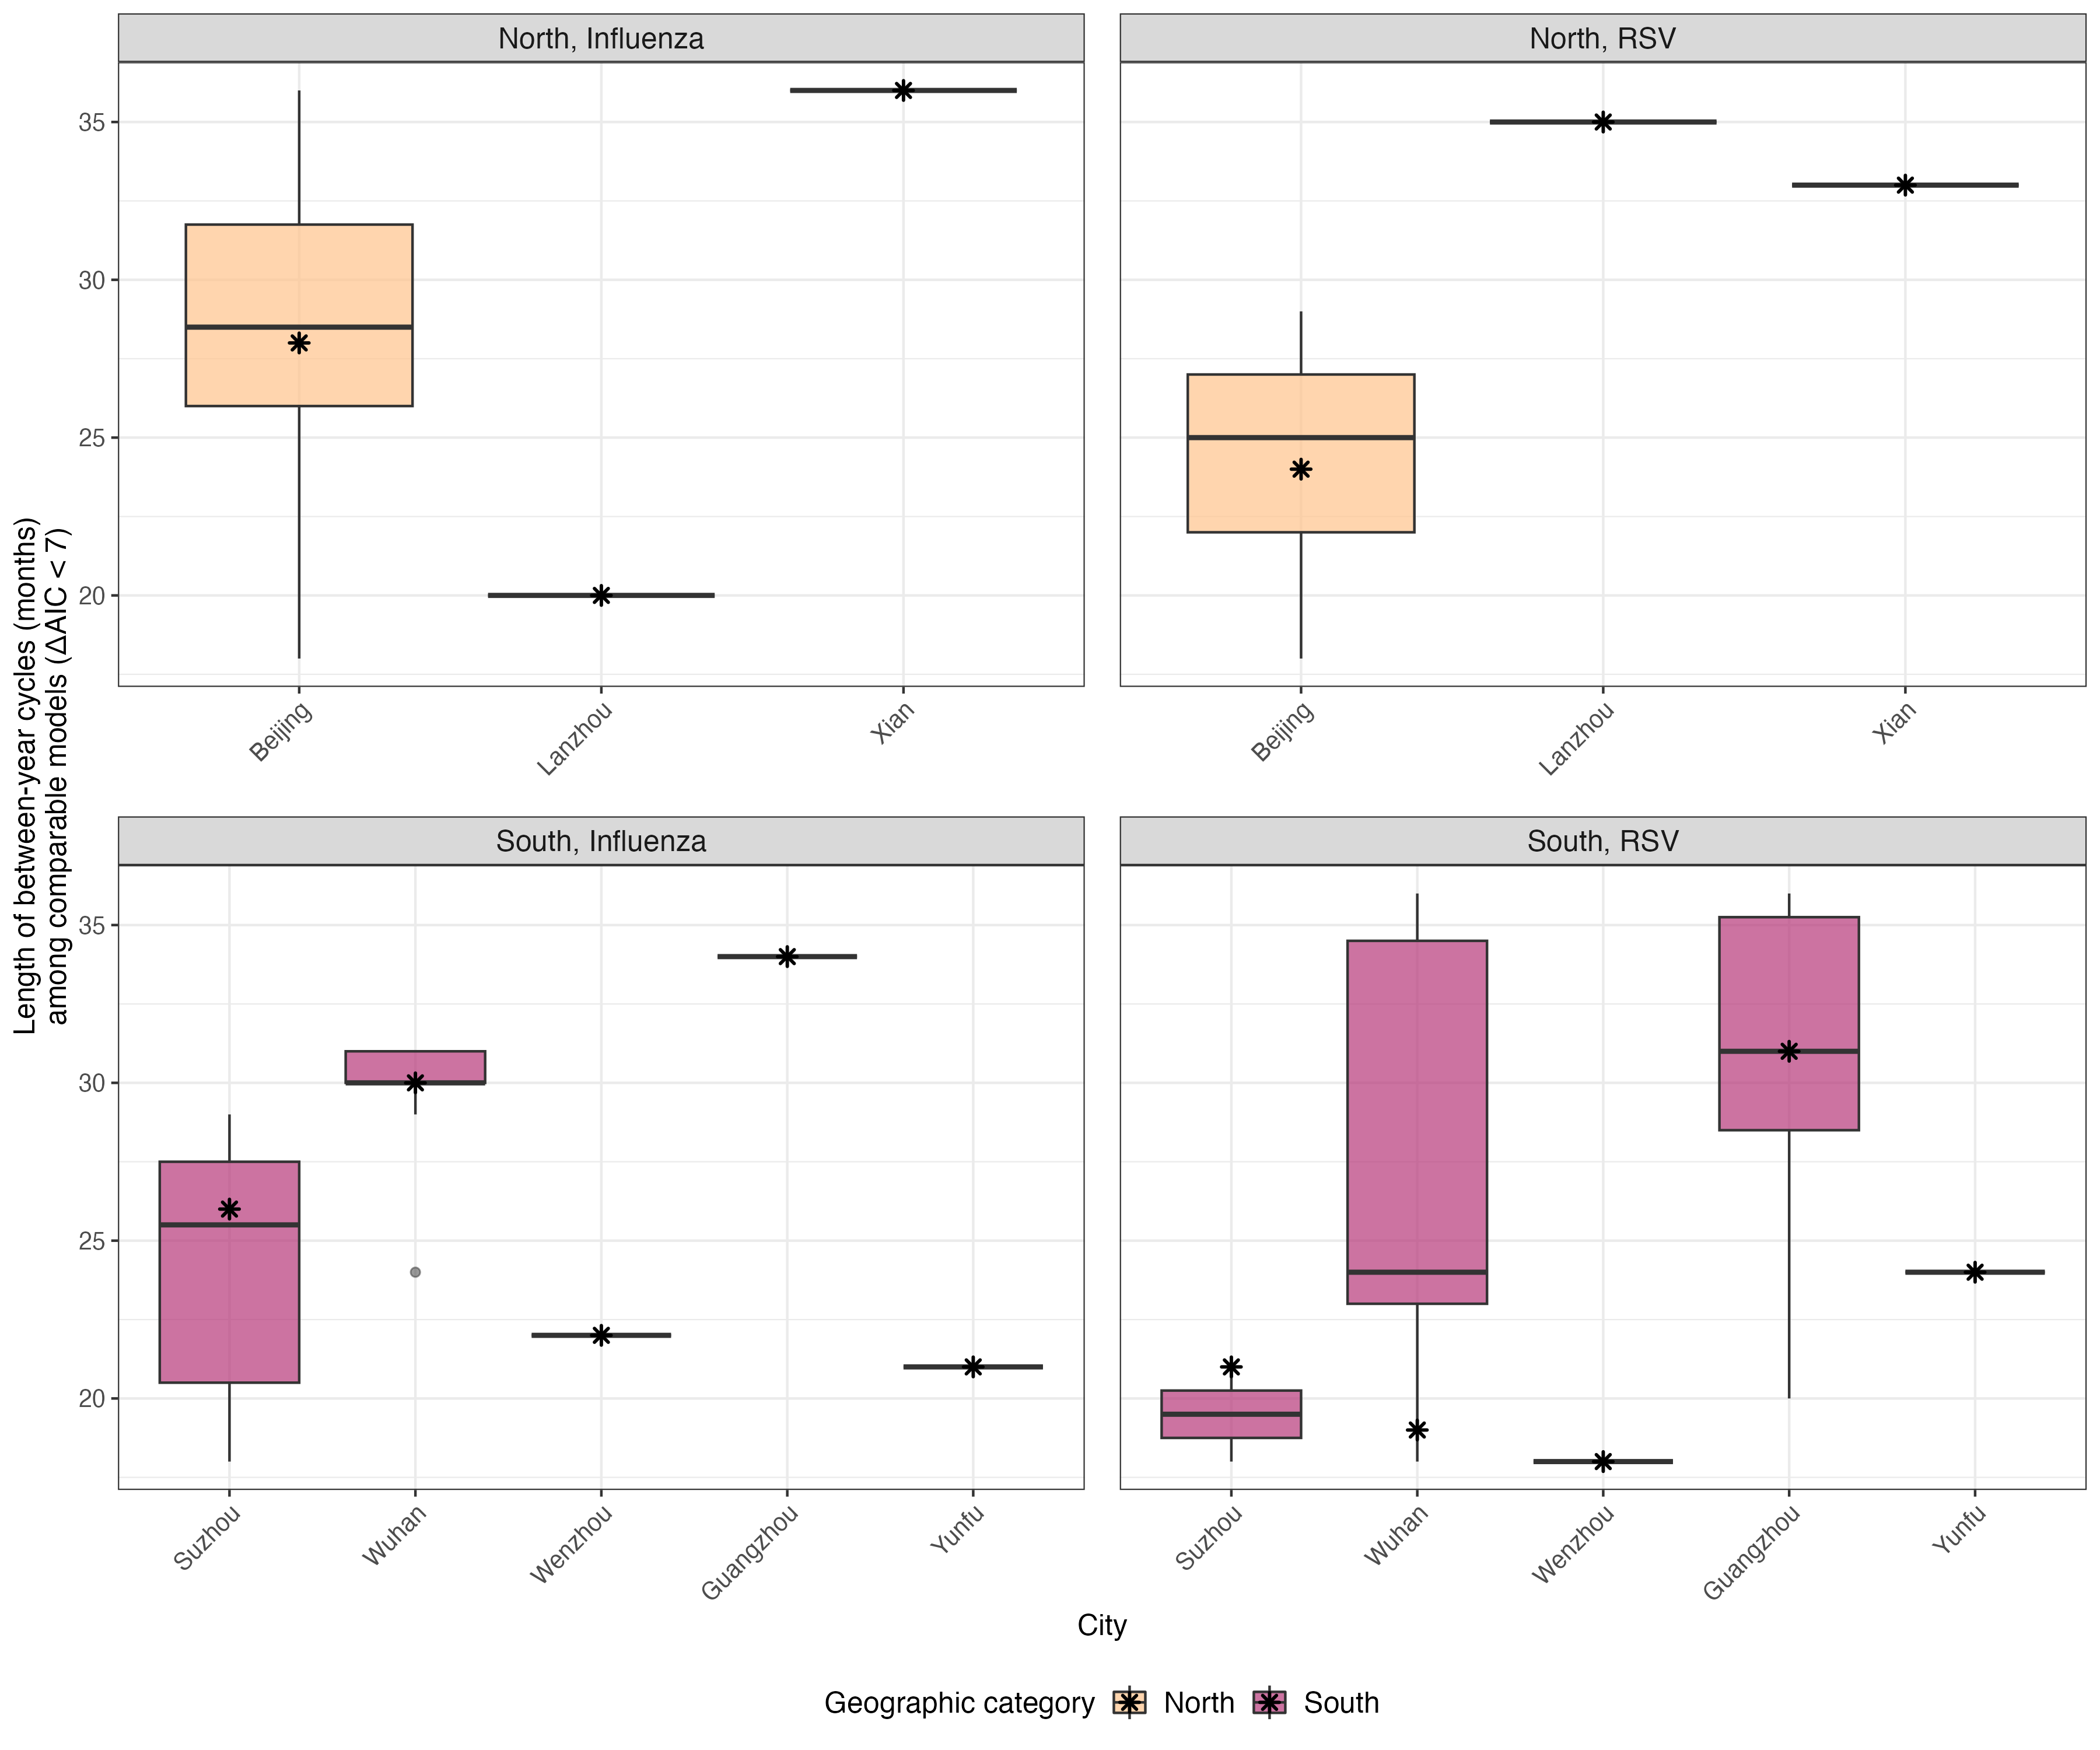
\includegraphics[width=0.9\textwidth]{../figures/supplemental_Figure1_threshold_7.png}
\caption{Figure S1: Distribution of between-year cycle lengths (months) among comparable models ($\Delta$AIC $< 7$) by city and pathogen, separated by geographic region (North vs South). Each panel displays boxplots of the between-year cycle lengths (in months) for each city within the specified region and pathogen combination. The asterisk (*) marks the best-performing model (lowest AIC) for each city-pathogen combination.}
\label{fig:supplemental_cycle_lengths}
\end{figure}

\clearpage

% ===== SUPPLEMENTARY TEXT SECTION =====
\section*{Supplementary Text 1. Literature search strategy}

We identified city-level surveillance data for respiratory syncytial virus (RSV) and influenza virus (InfV) through structured searches in PubMed. Searches were conducted on 12 August 2024, with no language restrictions. The full search strings and screening criteria are provided below.

\subsection*{RSV search}

The PubMed search string was:

\begin{verbatim}
("Respiratory Syncytial Viruses"[Mesh] OR RSV[Title/Abstract] 
 OR "respiratory syncytial"[Title/Abstract])
AND (China[Mesh] OR China[Title/Abstract] OR Chinese[Title/Abstract])
\end{verbatim}

Studies were included if they met all of the following criteria:
\begin{itemize}
    \item Surveillance data reported at the prefecture- or city-level (administrative level two);
    \item At least five consecutive years of observations;
    \item Monthly or weekly temporal resolution;
    \item Laboratory-confirmed RSV indicators (positivity among ARI/LRTI inpatients or outpatients).
\end{itemize}

Through this process, eight cities were identified with eligible RSV time series: Beijing, Lanzhou, Xi’an, Wuhan, Suzhou, Wenzhou, Guangzhou, and Yunfu.

\subsection*{Influenza search}

For the same eight cities, we applied a parallel PubMed search using the following query:

\begin{verbatim}
("Influenza, Human"[Mesh] OR influenza[Title/Abstract])
AND (China[Mesh] OR China[Title/Abstract] OR Chinese[Title/Abstract])
AND "last 10 years"[PDat]
\end{verbatim}

The same inclusion criteria were applied (prefecture-level data, ≥5 years of continuous observations, and monthly or weekly reporting). For cities with multiple eligible influenza series, we selected the dataset with the longest uninterrupted coverage and the most specific virological definition. Data sources corresponding to each city–pathogen pair are listed in Supplementary Table~S1.






\begin{table}[htbp]
    \centering
    \renewcommand{\arraystretch}{1.25}
    \begin{threeparttable}
    \caption{Supplementary Table S1. Surveillance indicator definitions for RSV and influenza (InfV) across included Chinese cities}
    \begin{tabular}{@{}llllll@{}}
    \toprule
    City & Pathogen & Indicator definition & Clinical setting & Laboratory method & Reference \\ 
    \midrule
    
    Beijing & RSV & RSV positivity among ARI inpatients & Inpatient (ARI) & IF on NPA & [a] \\
    Beijing & InfV & Influenza positivity in ILI cases & Outpatient (ILI) & Culture or throat swab PCR & [b] \\
    
    Xi’an & RSV & RSV positivity among ARI inpatients & Inpatient (ARI) & Antigen / mixed methods & [c] \\
    Xi’an & InfV & ILI case counts (syndromic) & Outpatient (ILI) & Not virological & [d] \\
    
    Lanzhou & RSV & RSV positivity among ARI inpatients & Inpatient (ARI) & PCR + sequencing (NPA) & [e] \\
    Lanzhou & InfV & Clinically diagnosed influenza cases & Outpatient/inpatient & Clinical diagnosis & [f] \\
    
    Wuhan & RSV & RSV positivity among ARI inpatients & Inpatient (ARI) & IF on NPA & [g] \\
    Wuhan & InfV & Influenza positivity in ILI cases & Outpatient (ILI) & RT-PCR & [h] \\
    
    Wenzhou & RSV & RSV positivity among LRTI inpatients & Inpatient (LRTI) & DFA on deep airway secretions & [i] \\
    Wenzhou & InfV & Influenza positivity in LRTI inpatients & Inpatient (LRTI) & IF on NPA & [j] \\
    
    Suzhou & RSV & RSV positivity in neonatal LRTI inpatients & Inpatient (LRTI, neonatal) & DFA on NPA & [k] \\
    Suzhou & InfV & Influenza positivity in SARI inpatients <5y & Inpatient (SARI) & RT-PCR on NPA & [l] \\
    
    Guangzhou & RSV & RSV positivity in ARI patients & In-/outpatient & qPCR on NP swabs & [m] \\
    Guangzhou & InfV & Influenza positivity in ILI outpatients & Outpatient (ILI) & PCR on throat swabs & [n] \\
    
    Yunfu & RSV & RSV positivity in pediatric inpatients & Inpatient (pediatric) & IF on NPA & [o] \\
    Yunfu & InfV & Influenza positivity in ILI outpatients & Outpatient (ILI) & Virus isolation + PCR & [p] \\
    
    \bottomrule
    \end{tabular}
    
    \begin{tablenotes}[flushleft]
    \footnotesize
    \item [a] Cui G et al. \textit{PLoS One}. 2013.
    \item [b] Wu S et al. \textit{Influenza Other Respir Viruses}. 2018.
    \item [c] Zhang L et al. \textit{Modern Preventive Medicine}. 2018.
    \item [d] Chen D et al. \textit{Entropy}. 2023.
    \item [e] Liang X et al. \textit{Medicine}. 2019.
    \item [f] Liu H-X et al. \textit{Dis Surveillance}. 2022.
    \item [g] Zhang X et al. \textit{Front Pediatr}. 2023.
    \item [h] Liu X et al. \textit{BMC Infect Dis}. 2023.
    \item [i] Lin J. Master's thesis, Wenzhou Medical University. 2011.
    \item [j] Zhong P-P et al. \textit{Chin J Contemp Pediatr}. 2016.
    \item [k] Lu L et al. \textit{BMC Infect Dis}. 2015.
    \item [l] Yu J et al. \textit{Pediatr Infect Dis J}. 2019.
    \item [m] Zou L et al. \textit{Front Microbiol}. 2016.
    \item [n] Yan Z-L et al. \textit{BMC Public Health}. 2024.
    \item [o] Qin C et al. \textit{China Practical Medicine}. 2022.
    \item [p] Peng L-X et al. \textit{Practical Preventive Medicine}. 2016.
    \end{tablenotes}
    
    \end{threeparttable}
    \end{table}
